\chapter{Conclusion}
% End-Ergebnisse und kritische Wertung
Overall, the team is satisfied with the project result. This was the first Kaggle challenge for all four members.
The team was able to place 975th out of a total 2065 participants, with a private score of 0.4977 on the already finished Kaggle competition leaderboard:
\vspace{1em}


\begin{figure}[H]
    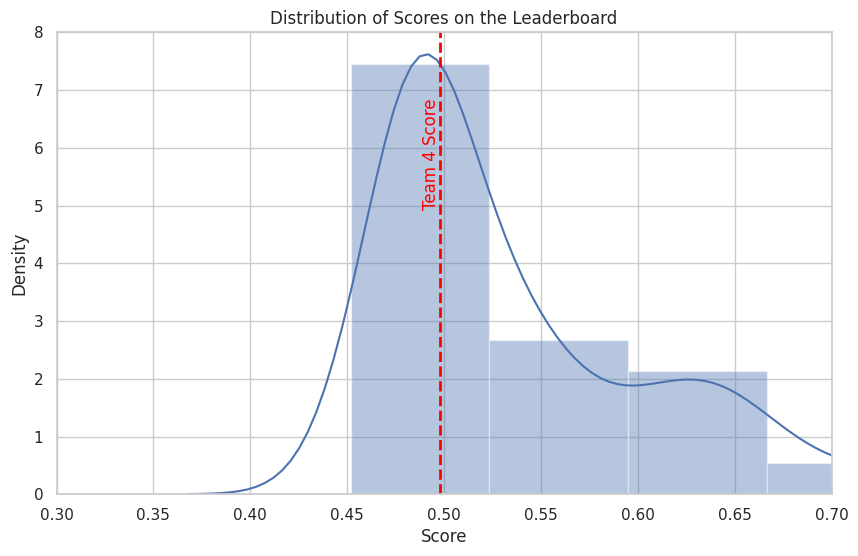
\includegraphics[keepaspectratio, width=\textwidth]{score_dist.png}
\caption{Kaggle Score Distribution}
\label{fig:score_dist}
\end{figure}
\vspace{1em}

\noindent When looking at the winning solution, it became apparent that developing a similar approach would be challenging due to the complexity and depth of the winner's strategy.
In summary, the leader used Large Language Models with specific prompts to augment data, coupled with a four-fold transformer ensemble.
\\

\noindent With the absence of time constraints and hardware limitations, the team could have explored additional approaches. This might have involved using a larger DeBERTa model or dedicating more time to the development of the ensemble. Nevertheless, the achieved results are considered satisfactory, given the unique solution employed.
The solution combines a deep-learning approach such as transformers and a linguistic approach 
such as \gls{rouge}-Based Model and LightGBM with linguistic features.

 





\section{Challenges and Lessons Learned}
At the beginning of the project, none of the team members had completed the Natural Language Processing course.
Instead, the NLP course was taken in parallel with the AI Challenge course.
This made it especially difficult to work with transformers, since they are quite an large topic to understand.
While on the topic on transformers, they are computationally intensive models and,
even with the provided hardware from the university, computing limitations were still an issue.
This was not the only challenge; the team also never worked with or implemented an ensemble.
Nevertheless, with these challenges the team has definitely learned a lot in the field of NLP and how machine learning in general can be used in real life settings.


\chapter{Reflection}
At the beginning of the challenge there was not a lot of motivation coming into the project.
When selecting the competition, we did not find a topic that seemed interesting to us and just settled for "Evaluate Student Summaries".
But as time went by, we grew to enjoy the challenge, especially after implementing our own ideas to solve the problem.
Communication within the team and with our coach was a strong point. We consistently received valuable feedback and could freely discuss machine learning queries. 
Our approach to planning was systematic, with weekly goals and milestones that kept us on track. Notably, our presentation skills noticeably imporved with each successive presentation.

\vspace{1em}

\noindent At the end of the day, we feel that the AI Challenge course served as a good preparation for the upcoming Bachelor Thesis
and are thankful for the opportunity as we are now more confident to write and present any technical project.
% Fazit zur Challenge & Lessons learned
